\section{Monday, March 10: Classification and Regression Trees}

This is one of my favorite topics! At first, this algorithm might seem like a totally ``new idea". But later, I hope you will see a lot of connections with algorithms we have already studied!

One note before we start: there are actually a lot of algorithms out there for building classification and regression trees! I will get to this in ``historical context." Whenever I don't say otherwise, if I am talking about a tree algorithm, assume that I am talking about the CART framework, which was popularized by Breiman et al. in 1984. 

\subsection{The main idea of the algorithm}

Let's start with some really basic motivation for a regression tree. At first glance, it might seem a bit different than the other methods we have seen in this class. 

The motivation begins with the left panel of Figure~\ref{fig_cart}. We have two covariates, $X_1$ and $X_2$. And then we have a numerical response variable $Y$. We begin the algorithm with the simplest possible model. This model just ignores the covariates and predicts $\hat{y} = \bar{y}$ for all observations. In this case, $\bar{y} = -2.6$. This is the ``intercept only" model. It has MSE given by: $\sum_{i=1}^n (y_i - \bar{y})^2$.

The algorithm then proceeds in a way that might remind you of forward stepwise regression. The algorithm says: at this moment in time, what is the binary split in my covariate space that will most improve the MSE, if I now let each sub-region be summarized by its own sample mean. This is illustrated in the second panel of Figure~\ref{fig_cart}. In this particular dataset, it turns out that the best way to chop our space into two is to draw a vertical line at $X_1 = -0.89$. Once we do this, any observation to the left of the split gets $\hat{y}=10$, and every observation to the right of the split gets $\hat{y}=-7$. This cutoff of $X_1 = -0.89$ was chosen greedily after considering all possible splits.

Let's write this down more rigorously. As of step 1 in the algorithm, our model has a single ``region" in it. This region is $R_0 = \mathbb{R}^p$: the whole covariate space. The set of possible splits are indexed by $j \in 1,\ldots,p$ and $s \in 1,\ldots, n$, where $x_{j,(s)}$ denotes the $s$th order statistic of the $j$th covariate\footnote{In the case of non-ordinal categorical $X_j$, we assign orders to the categories by sorting them by their average value of $Y$ in the training set. Thus, the order statistics are still defined; we just have a lot of ties in the order statistics: meaning that $x_{j,(1)}=x_{j,(2)}=x_{j,(3)}$ if all three observations belong to the same category.}. At the first level of the tree, we search exhaustively for:
\begin{equation}
\label{eq_SPLIT}
j^*, s^* = \argmax_{j \in 1,\ldots,p, s \in 1,\ldots n} Gain(R_0, j,s) = \sum_{i \in R_0} (y_i - \bar{y}_{R_0})^2 - \left( \sum_{i \in R_{L(j,s)}} (y_i - \bar{y}_{R_{L(j,s)}})^2  + \sum_{i \in R_{R(j,s)}} (y_i - \bar{y}_{R_{R(j,s)}})^2 \right),
\end{equation}
where $R_{L(j,s)} = \{ i \in R_0 : x_{j,i} \leq x_{j,(s)}\}$ and $R_{R(j,s)} = \{ i \in R_0 : x_{j,i} > x_{j,(s)}\}$. We refer to these as the regions to the left and the right of the split. Note also that $\bar{y}_R = \frac{1}{|i \in R|} \sum_{i \in R} y_i$ just denotes the sample mean of $y$ within a certain region. This was a lot of notation, but it can be worth it to make sure that you really understand what the algorithm is doing! But the idea is simple: we choose the split that most improves the MSE of our model right now. Alternate Gain functions are possible, but this MSE one is the one used by Breiman et al. (1984) in their very widely used CART algorithm. 

\begin{figure}[h]
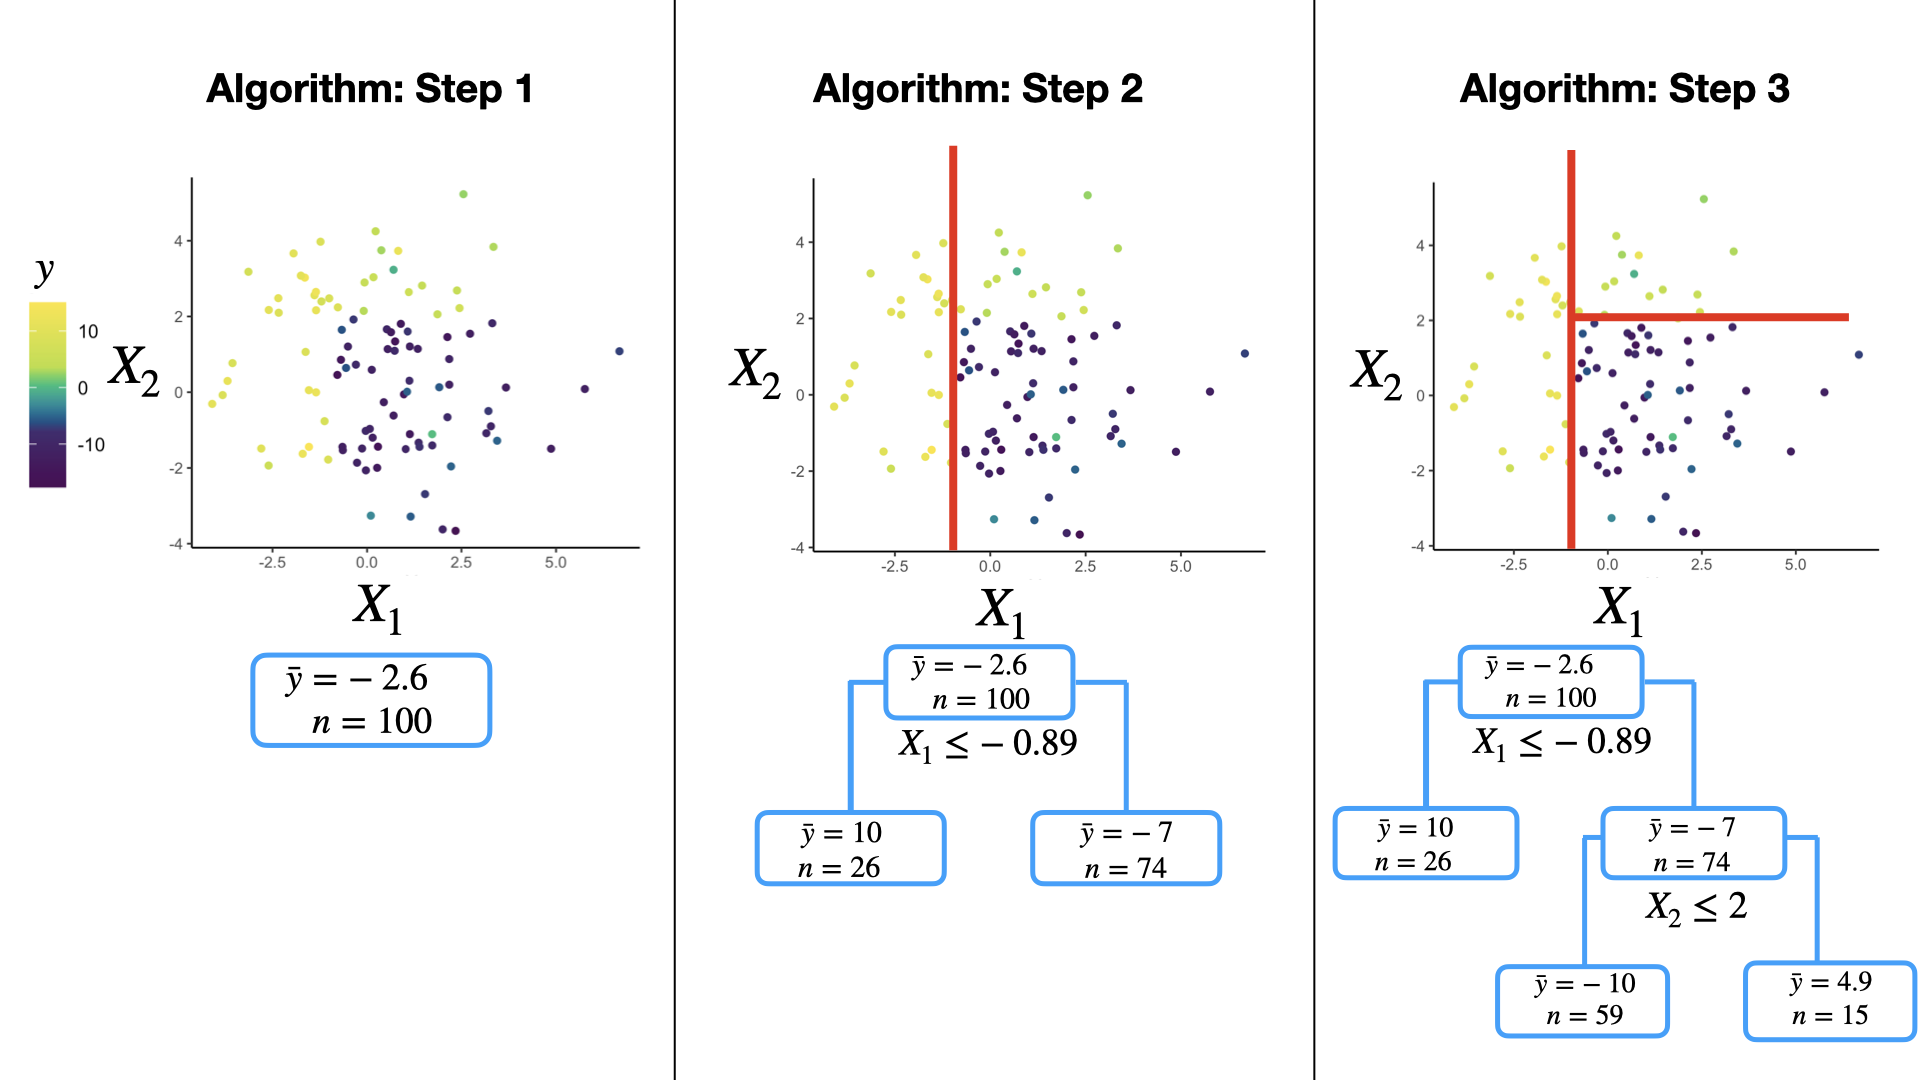
\includegraphics[width=0.9\textwidth]{442_lecs/CART_figure/CART_figure.001.png}
\caption{A little animation of the first three steps of a regression tree algorithm. Here, we have two covariates: $X_1$ and $X_2$. And then we have a numerical response variable $Y$. In this case, it seems like the data is generated from a ``true tree" structure, where there are rectangles in covariance space that define the average value of $Y$. The CART algorithm uses binary recursive partitioning to greedily search for the best possible rectangles, according to MSE!}	
\label{fig_cart}
\end{figure}

Finally, the right panel of Figure~\ref{fig_cart} shows what happens next. Regression trees are \emph{recursive partitioning algorithms}. So, the greedy search for the best possible splits, but now $R_0$ is replaced by the already-selected regions $R_{L(j^*,s^*)}$ and $R_{R(j^*,s^*)}$. We proceed until a stopping criteria is met.

The final model is a set of nested rectangles in covariate space. The prediction in each rectangle is just the sample mean of the training observations in that rectangle. We draw the model as a tree; as shown in Figure~\ref{fig_cart}. We write this model as:
$$
\hat{y} = \hat{f}(X) = \sum_{R \in \mathrm{TREE}} \bar{y}_R \bold{1}\{X \in R\}. 
$$
Sometimes the final regions in the tree are called leafs, and the series of splits that lead to them are called branches. This really leans into the tree analogy. I will just as often refer to them as terminal regions or terminal nodes, etc. 

We really have now gone over the main idea of trees! Now we will talk about some considerations and extensions. 

\subsection{Considerations, extensions, and historical context}

\subsubsection{Stopping criteria}

How do we know how big to build our tree? As you may have guessed, this is the main knob that controls our bias-variance tradeoff for trees. 

The biggest possible tree would keep splitting until we have one training observation per leaf region. This tree would have worst-case depth $n$, but likely depth closer to $log(n)$ if the tree remains more balanced. I think you all know that a tree like this will overfit severely to the training data, and we probably do not want to build this tree! We should stop before this! 

Some simple ideas for when to stop are to pre-specify the maximum depth of our tree, or the minimum node size in our tree (i.e. stop splitting when the region has less than 10 training observations in it). However, these are stopping criteria that do not adapt to the amount of signal in the data. The true ``right-sized" tree probably depends on the signal in our data! So, there are some more popular choices. 

Consider \eqref{eq_SPLIT}. What if we decided to not choose ANY split if this gain does not exceed some threshold? For example, if the MSE does not improve by more than 5\% when pick the best possible way to split this region, do not split this region at all. Such an idea is very similar to doing forward stepwise selection with an AIC or BIC stopping criteria. We recognize that ANY split will improve the training MSE *some*, but we want to make sure that the split seems ``worth it". In the \texttt{rpart} R package, this is controlled by the parameter \texttt{cp}. From the \texttt{rpart} documentation: ``any split that does not decrease the overall lack of fit by a factor of \texttt{cp} is not attempted. For instance, with anova splitting, this means that the overall R-squared must increase by \texttt{cp} at each step. The main role of this parameter is to save computing time by avoiding splits that are obviously not worthwhile." The default in \texttt{rpart} is 0.01, which is pretty small. This is an example of an \emph{adaptive stopping criteria}. 

Your textbook (ISL) calls the adaptive stopping approach above ``short-sided". The idea is that, due to the greedy nature of CART, it could be the case that no split will exceed the MSE threshold ``right now", but it could help us uncover an important interaction in the next level of the tree. So, it would be good to avoid stopping too early! 

Another idea is to grow a tree that is purposely too large, and then to \texttt{prune} splits away from the tree. More formally, let:
$$
L_\lambda(T) = \sum_{R \in T} \sum_{i \in R} (y_i - \bar{y}_R)^2 + \lambda |T|.
$$
This is a loss function that incorporates both tree MSE as well as a penalty term that penalizes larger trees: $|T|$ denotes the number of leaves in a tree. It turns out that nice properties of trees tell us that, if we start by building a large tree $T^{big}$, then there is a simple nested sequence of sub-trees that corresponds to the best tree for different values of $\lambda$. And we can find this sequence of trees easily: starting from $T^{big}$ we prune the ``weakest link" in the tree one at a time. This gives us the nested sequence of trees. This is a ``solution path"- like we had for Ridge or Lasso.  

To be really complete, we would want to use cross-validation to pick the best value of $\lambda$. And then we would want to re-fit a tree to the full training set using this value of $\lambda$. If you are not yet comfortable with the idea of cross validation + refitting to entire training set, please ask questions before the midterm! It is an important idea! 

\subsubsection{Categorical predictors}

CART can really seamlessly handle categorical predictors. We don't need to turn them into dummy variables!

The Breiman et al. CART algorithm always makes BINARY splits; even for categorical variables. You might encounter other decision tree algorithms some day that would make a three-legged-split for a categorical variable with three categories.

Ordinal categorical variables still have order statistics, so we split in the same manner than we did above in \eqref{eq_SPLIT}. For unordered categorical variables with $k$ categories, we do not need to consider $2^k$ possible ways to split the variable into two groups. We just order the categories by $\bar{y}$ on the training set, and then only let ourselves make a binary split that respects the ordering of these categories. 


NOTE: some critics of CART do not like the following fact. A numerical covariate has $O(n)$ chances to be chosen as the winning split. A binary categorical covariate has only 1 chance to be chosen as the winning split! If the binary covariate is truly important, but is associated with the numerical one, the numerical one will often appear in our tree! Just due to the extra random chance that it gets to be selected as a winner. This is too bad! There are modifications to the algorithm that try to get around this bias. 

\subsubsection{Categorical response}

CART is really easily used for either regression or classification.

For classification trees, all we do is modify our gain function. Instead of using MSE,  we split based on either Gini Index or Entropy. With either of these, we are choosing a split that makes the resulting child notes as pure as possible: meaning homogenous with respect to $y$. 

While we use Gini Index or Entropy to choose our splits greedily, we might still do cross validation using simple 0/1 classification error loss. 

\subsubsection{History}

I got some nice historical notes from this paper: \url{https://pages.stat.wisc.edu/~loh/treeprogs/guide/LohISI14.pdf}. 

The first classification tree algorithm was in 1963, and it was published under the name ``automatic interaction detection (AID)". This should already tell you something about why trees have been so popular- people absolutely love this feature that they can identify interactions without those interactions being pre-specified. At first, AID did not attract much attention from statisticians. People were worried about overfitting. People were also worried that, in the presence of correlated predictors, the conclusions could be spurious. Probably only one of the pair of correlated predictors will be selected for the tree, and the other will be totally left out. It might be dangerous to over-interpret the tree as signaling variable importance in that case\footnote{I agree!}. At the same time, however, computer scientists were making their own decision trees for ``concept learning." It seems that an early reference is Hunt, Marin, and Stone (1966). The algorithm that I learned about in CS class is ID3, which was published by Quinlan in a series of work in the 1980s. This is again a setting where great ideas were coming out concurrently in multiple disciplines!

The credit for ``popularizing" trees, at least in statistics, goes to Breiman et al. in 1984. I am pretty sure that one of the main innovations by Breiman et al. that really helped people take up trees was the introduction of efficient cost-complexity pruning. 

Since trees first became popular, there has been a lot more work on them! Some statisticians (including me) do not like that the splits in a CART tree lack a notion of statistical significance\footnote{This is very related to my claim, which we never finished going over, that you cannot easily do inference after stepwise regression. Greedily searching for optimal things makes inference hard.} One family of competing algorithms is called CTree; splits are chosen based on statistical significance, rather than based on an improvement in MSE. There are also models that make splits on linear combinations of variables, instead of single variables. Or models that fit an entire regression model to each leaf node, rather than choosing a piecewise constant model. And I am sure I am missing a lot of innovations! 

\subsection{What do we think about trees?}


\subsubsection{Bias}

An extremely large tree has almost no bias. We can approximate basically any function with a big combination of step functions. So if $n$ is big and our tree is big, trees are flexible. It is nice that trees can capture interactions between variables and other sorts of non-linear relationships without us needing to pre-specify.

However, a tree of reasonable size is very limited. Consider the case where $Y = 5 * X_1$. To approximate this well by a sequence of binary splits on the variable $X_1$, we will need a lot of splits! As we add more and more, our approximation will get better and better! But this function will obviously be much easier to approximate with a linear model!

In general, if the true data generating mechanism is not made up of rectangles in covariate space, a simple tree might struggle. But, if you are worried that rectangles in covariate space are REALLY biased, not that a really big tree works a lot like 1-NN, which we know does not have bias. See below for more about the connection to KNN. 

\subsubsection{Variance}

An extremely large tree has a lot of variance because it overfits. But even a small tree can have a lot of variance due to the greedy nature of trees. A small change to the input dataset can totally chance our first split, which could then affect our whole tree- especially if we only plan to make a small tree. So trees do not score super well for variance.

\subsubsection{Interpretability}

Trees are a dream! We can explain our predictions so easily to non-experts! Even things like interactions do not seem scary when they are presented as a tree! However, I have some notes below about a fundamental issue. If we know that our tree is unstable (high variance), what are we really interpreting? This makes formal inference really important. Which is something I worked on in my PhD!

\subsubsection{Use-ability}

Trees are a dream! They are ``off the shelf". The only tuning parameter is tree size, and tree size is something that we understand. And the nested-tree property of the pruning algorithm makes it really nice. 

We don't need to scale our predictors or worry about whether or not we are including an intercept. Categorical predictors need not be converted to binary. Missing data is also seamless to incorporate using the concept of surrogate splits. 
You don't need to start with preprocessing of variable selection. Trees do built in variable selection, and are not TOO impacted by curse of dimensionality. 

\subsubsection{Computational Efficiency}

When I first learned about trees, I thought that the algorithm sounded slow. Search exhaustively for best possible split? But now that I know about things like neural nets, I'm less concerned haha. Trees are pretty easy to implement. The greediness saves us. $O(np)$ things to compute at each level to choose a split. At least no squared terms, right? And the tree depth will be at MOST $n$, usually more like $log(n)$ if balanced. So maybe $O(np log(n))$. This really isn't bad. The pruning algorithm is also efficient. 

\subsection{Drawing connections!}

Right now, it might seem like decision trees are a random topic we have thrown in that are totally different from the other algorithms that we have seen. This is not true! Let's draw some connections.

\subsubsection{Write as a regression model or optimization problem}

Really, a regression tree defines a model class of piecewise constant models on rectangles in covariate space. So we could just abandon the whole tree idea and say that we are looking for a set of regions $R_1,\ldots, R_T$ such that we minimize
$$
L_\lambda(T) = \sum_{r=1}^T\sum_{i \in R_r} (y_i - \bar{y}_{R_r})^2 + \lambda |T|,
$$
and where $\hat{y} = \sum_{r=1}^T \bold{1}(X \in R_r) \bar{y}_{R_r}$. 

This looks a bit more like an optimization problem or a regression problem. We are regressing onto lots and lots of possible step-function indicator variables, but we are doing variable selection first to decide which ones to include. We can think of trees in this way! And then the innovation is just that this loss function will be really really difficult to minimize exactly. So, we give up on searching fully for the optimal tree. We instead use our greedy, top-down approach. Which finds a pretty good tree, but not necessarily the very best optimal tree. This reminds us of the difference between best-subset regression, which is infeasible, and stepwise regression, which is a greedy approximation.


\subsubsection{How is a regression tree like KNN?}

At the end of the day, the prediction $\hat{y} = \hat{f}(\xte)$ for a new datapoint $\xte$ is the sample mean of some training points $y$ that are near $\xte$ in covariate space. This sounds a lot like KNN! How is it different?
\begin{itemize}
\item In finding the points that are ``near" $\xte$, we do not consider all covariates $X_1,\ldots,X_p$. We only consider the ones that were selected for the tree. If we did a good job selecting splits for the tree, this should really help with the curse of dimensionality problem that KNN encountered. Irrelevant variables do not contribute! 
\item And we selected rectangles that lead to good predictions! So we should have retained important directions while ignoring irrelevant ones. 
\item We still have the ``prototype" interpretation: ``you got these predictions because other previous points in your rectangle 	had this average response." That is a really nice prediction! 
\item Overall, regression trees can maybe be seen as something that improves on KNN.
\end{itemize}

\subsubsection{Are regression trees parametric or non-parametric}

We just said that regression trees are kind of like stepwise regression (which is very parametric), but we also said that they are kind of like KNN (which is non-parametric). Which is it?

Remember that the definition of non-parametric is that our model complexity grows with our sample size $n$. As we said, the absolute biggest tree we can grow has $n$ leaves: one per training datapoint.

So, if we are building trees to unconstrained depth, then regression trees are non-parametric and are mode like KNN. Or, if we build trees with the restriction that the minimum node size is 10 but do no other pruning, then our model really is quite a bit like 10-NN. If we add more training datapoints, we can make more nodes, and so the complexity grows. Unless of course we run out of possible splits, which could happen if our variables are all categorical with not that many categories. 

However, if we build trees to a maximum depth of 3, then this is parametric and is a lot more like stepwise regression. We could enumerate the set of all possible models based on the size of our covariate space, and the models would not get more complex as we increase $n$; we would just get more observations per terminal node which reduces variance. Actually, we technically have more possible splits to choose from at each point when $n$ increases (order statistics), so if you want to be really precise about this being parametric imagine that your Xs are discrete and can take on only a set number of values. 

Overall, I think that the difference between fixed-depth trees and fixed-node-size trees as parametric vs. non-parametric models is interesting! And of course, adding in pruning changes the complexity again. You could study this yourself on a final project!

\subsection{Philosophically, can we really call an unstable model interpretable?}

I think there is a really important point when we talk about the pros and cons of decision trees. I will try to illustrate this point with my R demo.

Regression trees are supposedly so great because they are interpretable. But ... how do we know when we are seeing the truly important variables vs. seeing noise? We could also perturb our training dataset slightly and get a totally different tree, in the context of correlated predictors or similarly important predictors, etc. 

Isn't this really bad? What does it mean to interpret something that is unstable? We should probably add some notion of statistical significance to CART. Or work on making it more stable! This is the topic of a lot of research, including my own.  Let me know if you want references!





